\documentclass[varwidth=40cm]{standalone}
\usepackage{tikz}
\usetikzlibrary{calc}
\usepackage{style}

\let\r\undefined
\newcommand{\r}[2]{\draw[fill=lightgray] (#1,0) rectangle (#1+1,#2);}

\begin{document}
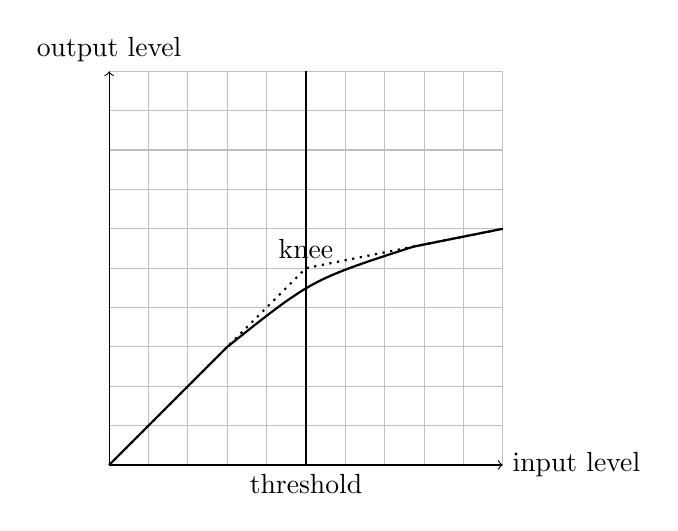
\begin{tikzpicture}[scale=0.5]
  \coordinate (a) at (3,3);
  \coordinate (b) at ({10-5*sqrt((sqrt(26)-2*sqrt(2))/11)},{6-sqrt((sqrt(26)-2*sqrt(2))/11)});
  \coordinate (ab) at ($(a)!0.5!(b)$);
  \foreach \i in {0,...,10} {
    \draw[lightgray] (0,\i) -- (10,\i);
    \draw[lightgray] (\i,0) -- (\i,10);
  }
  \draw (5,0) node[below] {threshold} -- (5,10);
  \draw[->] (0,0) -- (10,0) node[right] {input level};
  \draw[->] (0,0) -- (0,10) node[above] {output level};
  \draw[thick,dotted] (0,0) -- (5,5) -- (10,6);
  \draw[thick] (0,0) -- (a) .. controls ($(5,5)!0.4!(ab)$) .. (b) -- (10,6);
  \draw (5,5) node[above] {knee};
\end{tikzpicture}
\end{document}
